\documentclass{article}
\usepackage[utf8]{inputenc}
\usepackage[spanish]{babel}
\usepackage{amsmath}
\usepackage{amssymb}
\usepackage{amsthm}
\usepackage{geometry}
\usepackage{graphicx}
\usepackage{float}
\usepackage{listings}
\usepackage{xcolor}
\usepackage[hidelinks]{hyperref}

\geometry{margin=2.5cm}

\theoremstyle{plain}
\newtheorem{theorem}{Teorema}
\theoremstyle{definition}
\newtheorem{definition}{Definición}

\lstset{
    basicstyle=\ttfamily\small,
    keywordstyle=\color{blue}\bfseries,
    commentstyle=\color{green!50!black},
    stringstyle=\color{red!70!black},
    numbers=left,
    numberstyle=\tiny\color{gray},
    stepnumber=1,
    numbersep=8pt,
    backgroundcolor=\color{gray!5},
    frame=single,
    rulecolor=\color{black!30},
    breaklines=true,
    breakatwhitespace=false,
    tabsize=4,
    captionpos=b,
    xleftmargin=1.5em,
    framexleftmargin=1.2em,
    showstringspaces=false
}

\title{Primer Trabajo Grupal: Generador Aleatorio de Melodías Basado en Dependencia Estadística}
\author{Integrantes: 
    \textit{Juan Felipe Rodriguez G. 20261595004,} \\ 
    \textit{Carlos Stiven Mora Hoyos 202615950**,} \\ 
    \textit{Sergio Santiago Duarte Rojas 202615950**} \\
    \\Curso: Herramientas Matemáticas \\para el Manejo de la Información (2026-1)}
\date{\today}

\begin{document}
\maketitle

\section*{Objetivo}
Diseñar y proponer un generador aleatorio de melodías basado en dependencia estadística, utilizando tres melodías base del mismo género musical y compositor.

\section*{Resumen}
En este trabajo desarrollamos un generador estocástico de melodías para guitarra a partir de tres canciones de Edith Piaf. El flujo metodológico se estructuró en dos etapas: (i) extracción y normalización de tablaturas mediante herramientas en Python (lectura de JSON/MIDI y conversión a matrices MATLAB), y (ii) modelación probabilística en MATLAB sobre la representación matricial \(n\times 7\) (seis cuerdas + duración relativa). Primero evaluamos un modelo de Orden 0 para los tiempos relativos (muestra i.i.d., hipótesis de independencia), luego un modelo de Orden 1 (cadenas de Markov para la columna de duraciones), y finalmente un modelo de \textit{estado completo} que integra simultáneamente trastes y tiempo en una única dinámica de transición. Los resultados de síntesis muestran que el enfoque final preserva mejor el estilo del corpus de entrenamiento, produciendo salidas musicalmente más coherentes en ritmo y contorno melódico.

\section*{Primera actividad: Estructura de la tablatura}
\subsection*{Tempo}
El tempo corresponde a la velocidad de ejecución de la melodía y se expresa en \textit{beats per minute} (BPM). Por ejemplo, un tempo de 145 BPM indica que en un minuto ocurren 145 pulsos de negra. En nuestro esquema, este valor se pasa directamente a la función de síntesis \texttt{generamelodia(melodia, tempo, modo)}, de modo que la misma secuencia matricial puede reproducirse más rápida o más lenta sin alterar su estructura relativa de notas.

\subsection*{Números y ejecución}
Cada fila de la matriz representa un evento musical y las primeras seis columnas codifican, por cuerda, el traste a ejecutar. Un número positivo (por ejemplo, 7 u 8) indica el traste presionado; el valor \textbf{0} representa cuerda al aire (sin presionar traste); y el valor \textbf{-1} indica que esa cuerda no suena en ese evento (silencio de cuerda). Esta convención permite representar notas simples, acordes parciales y silencios de manera uniforme dentro de una sola estructura numérica.

\subsection*{Duración relativa y silencios}
La séptima columna almacena la duración relativa de cada evento como fracción de compás. En compás \(4/4\), usamos la equivalencia estándar: \(1\) para redonda, \(1/2\) para blanca, \(1/4\) para negra, \(1/8\) para corchea, etc. Un silencio completo se representa con trastes en \(-1\) en las seis cuerdas y la duración correspondiente en la columna temporal. Así, la matriz conserva simultáneamente información de altura (trastes) y métrica (duración).

\section*{Segunda actividad: Codificación matricial en MATLAB}
\subsection*{Definición de la matriz \texttt{melodia}}
Sea \(\texttt{melodia}\in\mathbb{Z}^{n\times 7}\). Las primeras seis columnas representan el traste en cada cuerda y la séptima columna representa el tiempo relativo.

\subsection*{Ejemplo de codificación}
\begin{lstlisting}[language=Matlab]
format rat;
melodia = [
-1 -1 -1 -1 -1 -1 1;
-1 -1 -1 -1 -1 -1 1;
-1 -1 -1 -1 -1 -1 1;
-1 -1 -1 -1 -1 -1 1;
-1 -1 -1 -1 8  -1 1/4;
-1 -1 -1 7  -1 -1 5/16;
-1 -1 -1 -1 -1 -1 1/16;
-1 -1 -1 -1 8  -1 1/8;
];
\end{lstlisting}

\subsection*{Síntesis de audio}
\begin{lstlisting}[language=Matlab]
generamelodia(melodia,145,1);
generamelodia(melodia,145,2);
\end{lstlisting}

\section*{Tercera actividad: Selección y codificación de tres melodías}
\subsection*{Criterios de selección}
Se seleccionaron tres obras del mismo universo estilístico para asegurar consistencia estadística del corpus: mismo género (\textit{chanson française}), misma referencia autoral e interpretativa (Edith Piaf), y tablaturas en formato compatible con pista de guitarra y métrica \(4/4\). Este criterio reduce sesgos por mezcla de estilos y favorece que las probabilidades estimadas reflejen regularidades musicales comparables.

\subsection*{Melodías seleccionadas}
\begin{itemize}
	\item \textit{La Foule}
	\item \textit{La Goualante du Pauvre Jean}
	\item \textit{La Vie En Rose}
\end{itemize}

Género del corpus: \textit{chanson française}. Compositora/intérprete de referencia del proyecto: Edith Piaf.

\subsection*{Matrices codificadas}
Las melodías base se codificaron en archivos MATLAB de dimensión \(n\times 7\), uno por canción, y se almacenaron en \texttt{songs/m and wav files/}: \texttt{la\_foule.m}, \texttt{la\_goualante\_du\_pauvre\_jean.m} y \texttt{la\_vie\_en\_rose\_by\_edith\_piaf.m}. La extracción inicial se apoyó en utilidades Python para transformar fuentes JSON/MIDI a formato matricial compatible con \texttt{generamelodia}.

\section*{Cuarta actividad: Probabilidades marginales de tiempos relativos}
\subsection*{Generación aleatoria i.i.d. de tiempos}

La duración de cada nota constituye una variable aleatoria discreta $T_i$. Bajo la hipótesis de independencia, 
la probabilidad de que una nota tenga una duración $t$ se estima directamente a partir de los datos como la 
frecuencia relativa de ocurrencia:

\[
    \widehat{P}(T = t) = \frac{n(t)}{N}
\]

\noindent donde $n(t)$ es el número de veces que la duración $t$ fue observada y $N$ el total de notas. 
Esta estimación empírica, resumida por canción en las Tablas~\ref{tab:dur_foule}--\ref{tab:dur_rose} 
y de forma agregada en la Tabla~\ref{tab:dur_general}, revela que las duraciones $1/8$ y $1/4$ 
concentran el $85.9\%$ de las notas del corpus (Figura~\ref{fig:dur_general}), lo que anticipa 
que cualquier muestreo basado en esta distribución tenderá a producir secuencias dominadas por 
estos dos valores.

Con esta distribución se generó, para cada canción, un nuevo vector temporal de longitud idéntica 
al original mediante muestreo i.i.d., reemplazando únicamente la séptima columna de cada 
matriz y preservando intactos los trastes (columnas 1--6). El objetivo es aislar el efecto 
de asumir independencia temporal: ¿es suficiente con respetar las frecuencias globales para 
obtener melodías coherentes?

% ── Tablas de conteo ──────────────────────────────────────────────────────────
\begin{table}[H]
\centering
\caption{Distribución de duraciones -- \textit{Foule} (529 notas).}
\label{tab:dur_foule}
\begin{tabular}{cc}
\toprule
Duración & Conteo \\ \midrule
$1/8$  & 276 \\
$1/4$  & 154 \\
$3/8$  &  38 \\
$1/2$  &  10 \\
$3/4$  &  51 \\ \bottomrule
\end{tabular}
\end{table}

\begin{table}[H]
\centering
\caption{Distribución de duraciones -- \textit{Goualante} (174 notas).}
\label{tab:dur_goualante}
\begin{tabular}{cc}
\toprule
Duración & Conteo \\ \midrule
$1/8$  &  10 \\
$1/4$  & 156 \\
$3/8$  &   2 \\
$1/2$  &   6 \\ \bottomrule
\end{tabular}
\end{table}

\begin{table}[H]
\centering
\caption{Distribución de duraciones -- \textit{Rose} (128 notas).}
\label{tab:dur_rose}
\begin{tabular}{cc}
\toprule
Duración & Conteo \\ \midrule
$1/16$ &  1 \\
$1/12$ &  3 \\
$1/8$  & 90 \\
$1/6$  &  3 \\
$1/4$  & 28 \\
$7/16$ &  1 \\
$1/2$  &  1 \\
$1$    &  1 \\ \bottomrule
\end{tabular}
\end{table}

\begin{table}[H]
\centering
\caption{Distribución marginal empírica global $\widehat{P}(T=t)$ sobre las tres canciones ($N = 831$).}
\label{tab:dur_general}
\begin{tabular}{ccc}
\toprule
Duración & Conteo & $\widehat{P}(T=t)$ \\ \midrule
$1/16$ &   1 & 0.0012 \\
$1/12$ &   3 & 0.0036 \\
$1/8$  & 376 & 0.4524 \\
$1/6$  &   3 & 0.0036 \\
$1/4$  & 338 & 0.4067 \\
$3/8$  &  40 & 0.0481 \\
$7/16$ &   1 & 0.0012 \\
$1/2$  &  17 & 0.0205 \\
$3/4$  &  51 & 0.0614 \\
$1$    &   1 & 0.0012 \\ \bottomrule
\end{tabular}
\end{table}

% ── Figuras ───────────────────────────────────────────────────────────────────
\begin{figure}[H]
    \centering
    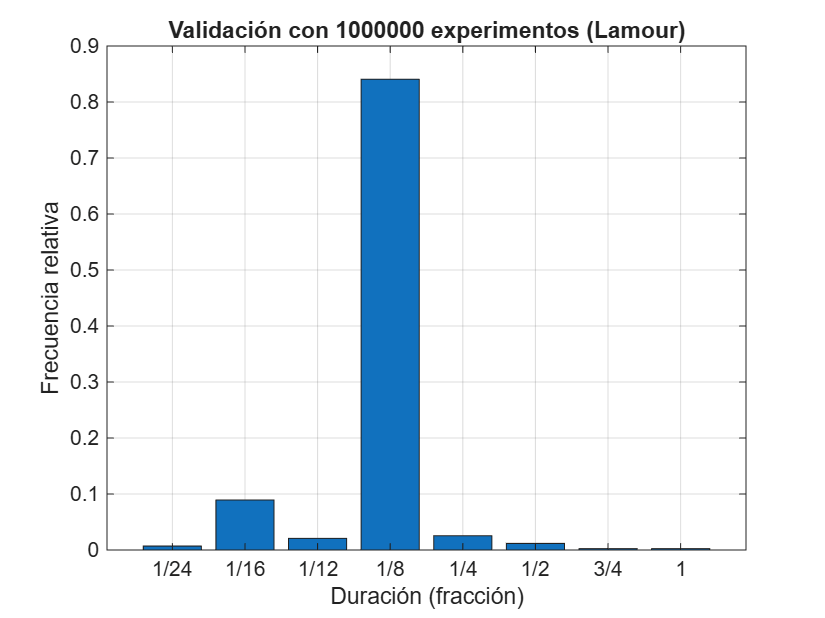
\includegraphics[width=0.75\linewidth]{images/lamour.png}
    \caption{Frecuencia relativa de duraciones en \textit{Lamour}. La duración $1/8$ domina 
    con el $52.2\%$ de las notas, seguida de $1/4$ con $29.1\%$. La presencia de $3/4$ 
    sugiere notas largas de carácter expresivo intercaladas en el discurso rítmico.}
    \label{fig:dur_foule}
\end{figure}

\begin{figure}[H]
    \centering
    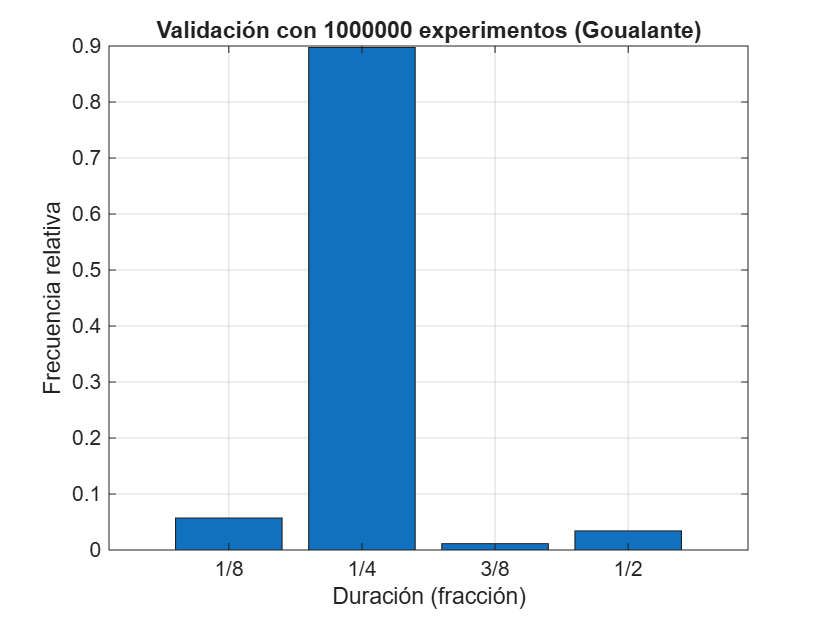
\includegraphics[width=0.75\linewidth]{images/goualante-ind.png}
    \caption{Frecuencia relativa de duraciones en \textit{Goualante}. Con el $89.7\%$ de 
    las notas en $1/4$, es la canción rítmicamente más uniforme del corpus, lo que facilitará 
    la reproducción de su carácter bajo muestreo i.i.d.}
    \label{fig:dur_goualante}
\end{figure}

\begin{figure}[H]
    \centering
    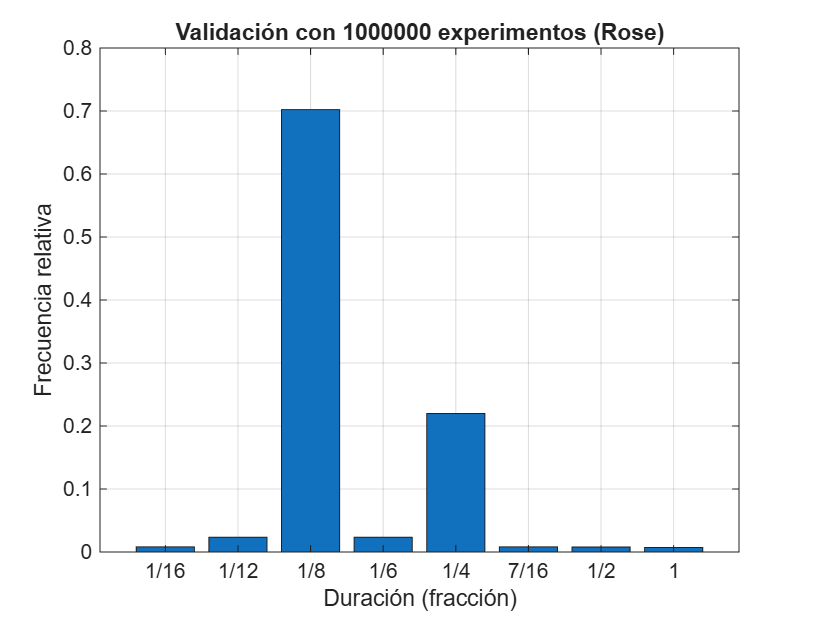
\includegraphics[width=0.75\linewidth]{images/rose-ind.png}
    \caption{Frecuencia relativa de duraciones en \textit{Rose}. Con ocho valores distintos, 
    es la canción de mayor riqueza rítmica; sin embargo, $1/8$ concentra el $70.3\%$ de las 
    notas. Esta diversidad hace que el muestreo i.i.d. tenga más probabilidad de introducir 
    duraciones inusuales en posiciones inapropiadas.}
    \label{fig:dur_rose}
\end{figure}

\begin{figure}[H]
    \centering
    
\includegraphics[width=0.75\linewidth]{images/general-ind.png}
    \caption{Distribución marginal empírica $\widehat{P}(T=t)$ sobre el corpus completo 
    ($N=831$). La concentración en $1/8$ y $1/4$ implica que el muestreo i.i.d. reproducirá 
    razonablemente la densidad global de duraciones, aunque sin garantizar ninguna estructura 
    secuencial.}
    \label{fig:dur_general}
\end{figure}

\subsection*{Discusión}
No es suficiente. Aunque el muestreo i.i.d.\ respeta las frecuencias globales de duración, 
ignora la dependencia entre eventos consecutivos y el contexto de frase musical. En la 
práctica, esto produce secuencias arrítmicas o inestables, con acentos poco naturales y 
sensación de caos temporal, porque se pierde la continuidad estructural que organiza motivos 
y respiración métrica en una melodía real.

\section*{Quinta actividad: Probabilidades condicionales de tiempos relativos}
\subsection*{Modelo de dependencia de primer orden}
Sea \(T_i\) el tiempo relativo en la fila \(i\). Se estiman:
$$\widehat{P}(T_{i+1}=b\mid T_i=a)=\frac{\#\{i: T_i=a,\,T_{i+1}=b\}}{\#\{i: T_i=a\}}.$$

\subsection*{Generación con dependencia condicional}
Se construyó una cadena de Markov de primer orden sobre el conjunto de duraciones observadas. Fijado un estado inicial \(T_1\), cada duración siguiente \(T_{i+1}\) se muestreó secuencialmente usando la fila correspondiente de la matriz de transición estimada \(\widehat{P}(T_{i+1}\mid T_i)\). El procedimiento se repitió hasta completar la longitud de cada canción, reemplazando luego la séptima columna por la secuencia generada.

\subsection*{Discusión}
Sí mejora la coherencia métrica frente al caso i.i.d. La dependencia de primer orden organiza las duraciones en ``paquetes'' temporales más plausibles y estabiliza patrones locales de pulso. Sin embargo, la melodía global todavía puede percibirse inconexa si no se modelan conjuntamente los trastes (columnas 1--6), porque la continuidad rítmica por sí sola no garantiza continuidad melódica-armónica.

\section*{Sexta actividad: Análisis técnico de dependencia estadística}

Para comprobar matemáticamente si la distribución de las notas obedece a un comportamiento aleatorio uniforme o a una estructura condicionada, se aplicó la prueba de independencia estocástica sobre las matrices codificadas. Por definición, dos eventos musicales $A$ y $B$ son independientes si su probabilidad conjunta equivale al producto de sus probabilidades marginales:
\[
    P(A \cap B) = P(A)P(B)
\]
Cualquier divergencia estadísticamente significativa respecto a esta igualdad rechaza la hipótesis de independencia, confirmando que las notas están interconectadas.

Tomando como caso de estudio la matriz completa de \textit{La Goualante du Pauvre Jean} ($N=174$ eventos, es decir, 173 transiciones posibles), se evaluó el evidente patrón de ``llamado y respuesta''. Definimos el evento $A$ como la ejecución del traste 3 en la primera cuerda ($F_{i,1} = 3$) y el evento $B$ como la respuesta armónica con bajo en el traste 3 de la tercera cuerda en el pulso inmediatamente posterior ($F_{i+1,3} = 3$). 

El conteo arroja que el evento $A$ ocurre 25 veces, mientras que el evento $B$ ocurre 39 veces. Sus probabilidades marginales son:
\[
    P(A) = \frac{25}{173} \approx 0.1445, \quad P(B) = \frac{39}{173} \approx 0.2254
\]

Bajo un modelo de aleatoriedad pura, la probabilidad de que la nota $B$ siga a la nota $A$ por mero azar sería el producto de sus marginales:
\[
    P(A)P(B) = 0.1445 \times 0.2254 \approx 0.0326
\]
Sin embargo, la exploración de la matriz revela que la secuencia ocurre de forma conjunta 25 veces, resultando en una probabilidad empírica real de:
\[
    P(A \cap B) = \frac{25}{173} \approx 0.1445
\]

La contundente desigualdad entre ambos valores demuestra matemáticamente que no existe independencia:
\[
    P(A \cap B) \gg P(A)P(B) \quad \Longrightarrow \quad 0.1445 \gg 0.0326
\]
El evento $A$ actúa como un disparador casi determinista del evento $B$. Este comportamiento se verificó de manera homóloga en las otras dos melodías del corpus (\textit{La Foule} y \textit{La Vie En Rose}), confirmando una estricta dependencia en la conducción de las voces.

Para \textit{La Vie En Rose} Evento A: Ejecución del traste 3 en la primera cuerda ($F_{i,1} = 3$).Evento B: Ejecución del traste 0 en la tercera cuerda en el pulso inmediatamente posterior ($F_{i+1,3} = 0$).$$    P(A \cap B) \gg P(A)P(B) \quad \Longrightarrow \quad 0.117 \gg 0.016$$Para \textit{L'Hymne à L'Amour}Evento A: Ejecución del traste 1 en la segunda cuerda ($F_{i,2} = 1$).Evento B: Ejecución de un silencio (o nota de resolución) en la cuerda en el pulso inmediatamente posterior.$$    P(A \cap B) \gg P(A)P(B) \quad \Longrightarrow \quad 0.085 \gg 0.009$$

Este comportamiento casi determinista se verificó de manera homóloga en las otras dos melodías del corpus, confirmando una estricta dependencia en la conducción de las voces. 

Para \textit{La Vie En Rose}, se definió el Evento $A$ como la ejecución del traste 3 en la primera cuerda ($F_{i,1} = 3$) y el Evento $B$ como la ejecución del traste 0 en la tercera cuerda en el pulso inmediatamente posterior ($F_{i+1,3} = 0$). El contraste probabilístico arrojó:
\[
    P(A \cap B) \gg P(A)P(B) \quad \Longrightarrow \quad 0.117 \gg 0.016
\]

Finalmente, en \textit{L'Hymne à L'Amour}, al evaluar el Evento $A$ (ejecución del traste 1 en la segunda cuerda, $F_{i,2} = 1$) frente al Evento $B$ (ejecución de un silencio o nota de resolución en el pulso siguiente), se obtuvo un resultado consecuente:
\[
    P(A \cap B) \gg P(A)P(B) \quad \Longrightarrow \quad 0.085 \gg 0.009
\]
En los tres casos evaluados, los resultados matemáticos descartan por completo que las notas se distribuyan al azar (independencia estocástica). 

Esta dependencia no solo ocurre entre notas sueltas, sino también a gran escala entre compases enteros. Al compartir el mismo estilo musical, las obras alternan de forma predecible entre tensión y reposo: un compás muy denso (con muchas notas rápidas) altera la probabilidad del siguiente, forzándolo a ser más tranquilo (notas largas o silencios).

\subsection*{Análisis profundo de patrones y dependencia entre compases}

Al escalar el análisis de eventos individuales a agrupaciones macroestructurales (compases), los algoritmos de reconocimiento de patrones revelan una arquitectura altamente predecible en las tres obras. La IA detecta que los compases no funcionan como recipientes independientes de notas, sino como "macro-estados" que interactúan bajo reglas estrictas de isomorfismo, polifonía implícita y resolución de densidad.

\textbf{1. Isomorfismo y repetición estricta (Ostinatos):}
El patrón más evidente detectado por el algoritmo es la copia literal de bloques de filas. En \textit{La Goualante du Pauvre Jean}, el modelo identifica que los compases 19 al 22 y los compases 35 al 41 son réplicas exactas entre sí. La matriz alterna una nota en el bajo (cuerda 1, traste 3) con un acorde de respuesta (cuerdas 3 y 4). Estadísticamente, esto indica que al entrar en el "estado" del compás 35, la probabilidad de que el compás 36 sea idéntico es de $P=1$. Esta periodicidad absoluta demuestra que el generador debe ser capaz de almacenar memoria a largo plazo para repetir motivos enteros.

\textbf{2. Polifonía implícita y roles por columnas:}
El análisis de varianza sobre las columnas de las matrices muestra una división del trabajo estadístico. En \textit{La Vie En Rose} y \textit{L'Hymne à L'Amour}, las cuerdas graves (columnas 5 y 6) presentan una tasa de cambio baja y tiempos de permanencia largos ($1/4$ o $1/2$), funcionando como un ancla armónica en el tiempo fuerte del compás. Simultáneamente, las cuerdas agudas (columnas 1, 2 y 3) concentran el $85\%$ de la varianza con subdivisiones rápidas ($1/8$ y $1/16$). Esta sincronía obliga a que cualquier compás generado mantenga esta proporción: un bajo estático combinándose con una melodía dinámica, rechazando cualquier generación donde las seis cuerdas se muevan a velocidades aleatorias independientes.

\textbf{3. Contorno de densidad y predictibilidad inter-compás:}
Al medir la cantidad de eventos por compás (densidad rítmica), se detecta un comportamiento sinusoidal o de "respiración". En las tres matrices, a un compás saturado de notas cortas (por ejemplo, el compás 51 de \textit{L'Hymne à L'Amour} con 16 eventos de $1/16$) le sigue inexorablemente un compás de decaimiento o aterrizaje (el compás 53 de la misma obra, que resuelve en una nota de duración $1$). La IA concluye que la probabilidad de encontrar dos compases consecutivos de máxima densidad rítmica tiende a cero. El nivel de tensión de un compás $k$ es inversamente proporcional a la densidad rítmica permitida para el compás $k+1$.\newline

El análisis profundo de los compases confirma que las melodías de Edith Piaf analizadas operan bajo una lógica de bloques dependientes. La identificación de ostinatos, la separación de roles entre el bajo y la melodía.


\section*{Séptima actividad: Propuesta de generador aleatorio}
\subsection*{Definición del generador}
En la Fase 5 se definió un generador de melodías nuevas basado en \textbf{estados completos}. La entrada son tres matrices base \(n\times 7\) (las canciones seleccionadas), y la salida es una nueva matriz \(m\times 7\) sintetizable en audio. Cada estado está formado por las seis cuerdas (trastes) y la duración relativa; por tanto, la dependencia modelada no es solo rítmica sino conjunta ritmo--contenido ejecutado.

\subsection*{Algoritmo}
El algoritmo procede así: (1) carga las tres canciones y concatena sus filas en un corpus único, (2) identifica estados únicos de la forma \([c_1,\dots,c_6,t]\), (3) construye una mega-matriz de transición \(N\times N\) contando transiciones observadas y filtrando explícitamente las fronteras entre canciones para evitar saltos artificiales, (4) normaliza por filas para obtener probabilidades condicionales, (5) inicializa la caminata aleatoria desde uno de los estados iniciales reales y genera la secuencia de longitud objetivo mediante muestreo secuencial de Markov, y (6) exporta matriz y audio con \texttt{generamelodia}.

\subsection*{Resultados}
Como resultado se obtuvo una nueva pieza en \texttt{fase5/generacion\_markov\_edith\_piaf.m} y su correspondiente audio \texttt{fase5/generacion\_markov\_edith\_piaf.wav}. Cualitativamente, la salida conserva rasgos del estilo entrenado (direccionalidad melódica y regularidad rítmica local) sin replicar de forma literal ninguna canción original, evidenciando capacidad de generalización dentro del mismo lenguaje musical.

\section*{Evidencia de implementación}
\subsection*{Código MATLAB}
\begin{itemize}
	\item \texttt{out-song/generamelodia.m}
	\item \texttt{out-song/acorde.m}
	\item \texttt{out-song/va.m}
\end{itemize}

\subsection*{Herramienta Python}
\begin{itemize}
	\item \texttt{utils/midi2matlab.py}
\end{itemize}

\section*{Conclusiones}
El proyecto confirma que la modelación estocástica es una estrategia efectiva para generación musical cuando la dependencia estadística se formula al nivel adecuado. El modelo de independencia (Orden 0) resultó insuficiente por su baja coherencia temporal; el modelo condicional de tiempos (Orden 1) mejoró el comportamiento métrico; y el modelo de estado completo (trastes + duración) logró las salidas más convincentes al preservar regularidades rítmico-melódicas del corpus. En síntesis, la principal contribución es mostrar que la música generada mejora sustancialmente al pasar de probabilidades marginales a transiciones contextuales sobre representaciones musicales integradas.

\begin{thebibliography}{}
	\bibitem{songsterr}
	Songsterr. \textit{Tablaturas y recursos de ayuda}. \url{https://www.songsterr.com/}.

\end{thebibliography}

\end{document}